% !TeX root = ../main.tex
\documentclass[./../main.tex]{subfiles}

\begin{document}
\section{Đặt vấn đề}
Hiện nay, phương thức tấn công phổ biến nhất đối với các tệp PDF độc hại bắt nguồn từ việc nhúng các đoạn mã javascript - những đoạn mã mà sẽ được thực thi bởi ứng dụng đọc tệp PDF. Lợi dụng nhiều lỗ hổng bảo mật nghiêm trọng từ các trình đọc PDF, có thể kể đến nhiều nhất là Acrobat Reader, các kẻ tấn công đã sử dụng mã javascript để thực hiện khai thác các lỗ hổng đó, nhằm xâm nhập vào hệ thống máy tính nạn nhân và thực hiện những hành vi độc hại. Việc phân tích tĩnh và trích xuất các đặc trưng thực hiện ở chương 2 chỉ mang tính chất thống kê và kiểm tra sự tồn tại của javascript, chưa thực sự đi sâu vào khai thác các hành vi của mã. Bên cạnh đó, với sự phát triển của kỹ thuật làm rối, các đoạn mã javascript càng trở nên khó phát hiện hơn, hoặc được xây dựng trông như một đoạn mã lành tính, gây nhiễu cho các mô hình phân loại học máy. Có thể thấy các đặc trưng đã trích xuất chưa thực sự đem lại một kết quả tốt với các mã có nhúng javascript.
Ở chương này, tôi đề xuất một phương pháp gồm hai giai đoạn để xử lý các tệp PDF có chứa javascript.
\begin{itemize}
	\item Giai đoạn một thực hiện trích xuất đặc trưng cơ bản và đưa qua bộ phân loại Zero False Positive với mục tiêu của giai đoạn này là tạo nên một tường lửa nhạy bén với các tệp độc, đảm bảo loại bỏ được những tệp chắc chắn là độc, tức mô hình học máy không gây ra dương sai (FP).
	\item Giai đoạn hai được đề xuất sẽ xử lý các tệp PDF được gán nhãn sạch, bằng các kỹ thuật xử lý nâng cao, đòi hỏi thời gian và chi phí phân tích hơn để tìm ra chính xác tệp PDF độc hại nào còn sót lại.
\end{itemize}

\section{Bộ phân loại Zero False Positive}
Bộ phân loại Zero False Positive được đề xuất trong giai đoạn một để mang tới một kết quả phân loại không có gán nhãn dương sai. Ý tưởng xây dựng dựa trên mô hình được đề xuất trong công bố của Mohammad Sayad Haghighi và cộng sự \cite{zfp}.

\subsection{Thuật toán phân loại lặp với mục tiêu FP = 0}
% figure
\begin{figure}[ht!]
	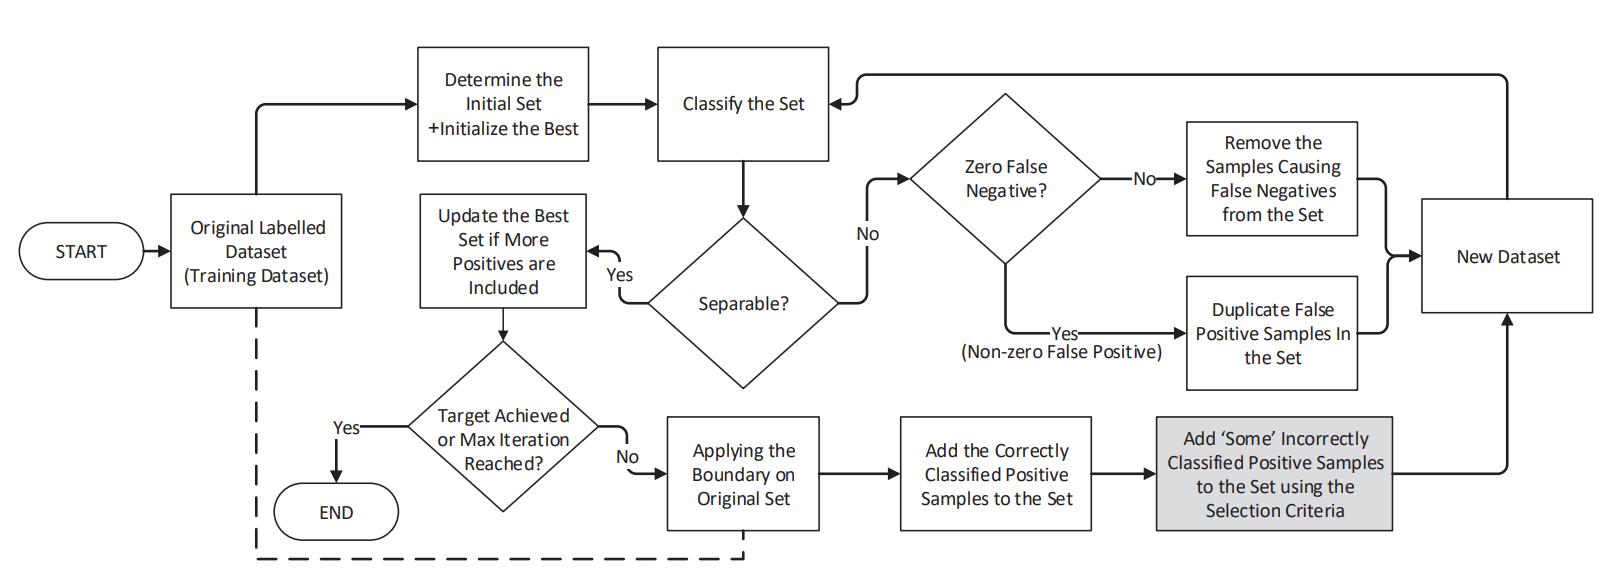
\includegraphics[width=\linewidth]{./images/zfp_flow_chart.png}
	\caption{Sơ đồ luồng hoạt động của thuật toán lặp Zero False Positive}
	\label{fig:zfp_flow_chart}
\end{figure}

% figure
\begin{figure}[ht!]
	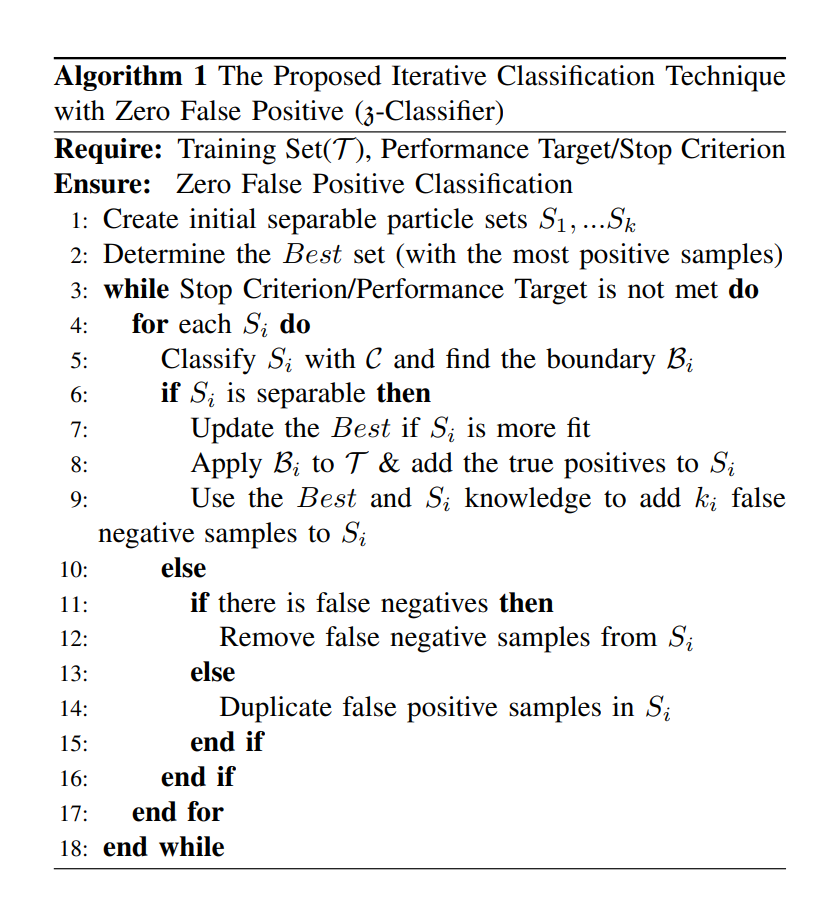
\includegraphics[width=\linewidth]{./images/algorithm_zfp.png}
	\caption{Mã giả thuật toán lặp Zero False Positive}
	\label{fig:algorithm}
\end{figure}
Thuật toán là kỹ thuật phân loại lặp với mục tiêu tỷ lệ phát hiện sai cho lớp dương là bằng 0 (tức không có mẫu âm nào bị phát hiện thành mẫu dương), dựa trên thuật toán Tối ưu bầy đàn \cite{swarm}. Từ một tập dữ liệu ban đầu, sẽ tạo ra nhiều các tập giản lược, được gọi là tập thành phần. Mỗi tập giản lược sẽ bao gồm tất cả các mẫu âm và một vài mẫu dương.
Mỗi tập thành phần bắt đầu với một tập giản lược mà được trích xuất từ tập huấn luyện ban đầu T bằng cách loại bỏ một số mẫu dương để có thể trở nên tách được (tức FP và FN bằng 0). Ở trường hợp lý tưởng, tập khởi tạo này chỉ có 1 mẫu dương và tất cả là mẫu âm. Cho trước một bộ phân loại C, chúng ta có thể thực hiện phân loại trên tập T ban đầu, và sử dụng những mẫu dương được phân loại đúng để tạo ra các tập khởi tạo.
Mỗi tập giản lược sẽ đi qua bộ phân loại C. Trong mỗi vòng lặp, nếu kết quả cho thấy sự tách được của tập (FP = 0 và FN = 0), tập sẽ được so sánh với kết quả tốt nhất trước đó của các tập thành phần khác, gọi là Best. Sự so sánh có thể là một hàm được định nghĩa trước ví dụ chứa bao nhiêu mẫu dương khi chúng ta muốn giảm số lượng FN. Nếu tập giản lược của tập thành phần mang lại số điểm tốt hơn, Best sẽ được thay thế.
Từ đó, biên mới của mô hình sẽ được dùng để phân loại lại tập dữ liệu ban đầu (như một tập kiểm thử). Theo đó,
Các mẫu dương được phân loại đúng sẽ được thêm vào tập thành phần Si cho vòng lặp tiếp theo.
Ngoài ra các mẫu dương bị phân loại sai (gây FN) sẽ được chọn lọc một phần (k mẫu) để thêm vào Si bằng cách sử dụng phương pháp Lựa chọn ngẫu nhiên dựa trên trọng số trên Best. Bởi những mẫu dương trong tập giản lược của Best sẽ có thể có trọng số, tức độ ưu tiên cao hơn.
Ở một trường hợp khác, thông qua các vòng lặp, nếu một tập thành phần trở nên không phân tách được tại một số điểm (ở đây là FP khác 0), thì sẽ được thông qua một quá trình cắt tỉa (pruning operation). Sự cắt tỉa này ban đầu sẽ được thực hiện bằng việc loại bỏ những mẫu dương mà gây nên phân loại âm sai (FN > 0). Nếu cách này không mang lại hiệu quả (sẽ được kiểm tra trong vòng lặp tiếp theo) hoặc không mang lại FP = 0, trọng số của các mẫu âm gây nên FP sẽ được tăng lên - bằng cách nhân bản các mẫu âm này trong tập thành phần. Có thể thấy, tập giản lược của tập thành phần có thể không nhất thiết là một tập con của tập huấn luyện T ban đầu. Quá trình cắt tỉa sẽ tiếp tục qua các vòng lặp cho đến khi tập này trở nên phân tách lại một lần nữa.
Toàn bộ quá trình thêm/ loại bỏ sẽ kết thúc khi hoặc đạt được mục tiêu FN (luôn muốn FN nhỏ nhất có thể) hoặc đã đạt số vòng lặp cho phép tối đa.


\subsection{Thực nghiệm và đánh giá kết quả}
Tiến hành thực nghiệm để kiểm định mô hình trên tập huấn luyện gồm các tệp PDF đã được trích xuất đặc trưng thống kê và đặc trưng cấu trúc trong chương 2. Kết quả cho thấy số lượng FP qua các vòng lặp đều được đảm bảo bằng 0 và số lượng FN giảm dần. Tuy nhiên, từ vòng lặp thứ 700 - 1000, kết quả FN không giảm, duy trì số lượng 97, với tỉ lệ FNR bằng 0.0095 (Bảng \ref{tab:ket_qua_thuat_toan_phan_loai}).

\begin{table}[]
	\centering
	\caption{Kết quả của thuật toán phân loại Zero False Positive trên tập dữ liệu đã trích xuất}
	\label{tab:ket_qua_thuat_toan_phan_loai}
	\begin{tabular}{|c|c|c|c|c|}
		\hline
		\textbf{Iteration} & \textbf{TN} & \textbf{FP} & \textbf{FN} & \textbf{TP} \\ \hline
		0                  & 7423        & 0           & 2993        & 7220        \\ \hline
		5                  & 7423        & 0           & 361         & 9852        \\ \hline
		10                 & 7423        & 0           & 255         & 9988        \\ \hline
		50                 & 7423        & 0           & 133         & 10080       \\ \hline
		100                & 7423        & 0           & 107         & 10106       \\ \hline
		200                & 7423        & 0           & 105         & 10108       \\ \hline
		500                & 7423        & 0           & 100         & 10113       \\ \hline
		700                & 7423        & 0           & 97          & 10116       \\ \hline
		1000               & 7423        & 0           & 97          & 10116       \\ \hline
	\end{tabular}
\end{table}

Ngoài ra, mô hình được tiến hành thử nghiệm trên một số tập dữ liệu khác. Bộ dữ liệu đặc trưng tệp PDF được trích xuất và công bố bởi đội ngũ phát triển Hidost \footnote{\url{https://github.com/srndic/hidost-reproduction}} với một số lượng lớn các mẫu PDF độc hại được thu thập qua nhiều năm. Tôi đã liên hệ Nedim Srndic, một trong những tác giả của Hidost \cite{hidost} để xin phép sử dụng bộ dữ liệu đặc trưng trong phạm vi khóa luận này. Bộ dữ liệu được phân thành nhiều tập, và dưới đây là kết quả của hai tập dữ liệu khi thử nghiệm trên mô hình phân loại Zero False Positive.

\begin{table}[]
	\centering
	\caption{Kết quả thuật toán phân loại Zero False Positive trên tập dữ liệu Hidost (1)}
	\label{tab:ket_qua_thuat_toan_phan_loai_hidost}
	\begin{tabular}{|c|c|c|c|c|}
		\hline
		\textbf{Iteration} & \textbf{TN} & \textbf{FP} & \textbf{FN} & \textbf{TP} \\ \hline
		0                  & 142796      & 0           & 1851        & 4406        \\ \hline
		10                 & 142796      & 0           & 410         & 5847        \\ \hline
		50                 & 142796      & 0           & 287         & 5970        \\ \hline
		100                & 142796      & 0           & 272         & 5985        \\ \hline
		120                & 142796      & 0           & 271         & 5986        \\ \hline
		160                & 142796      & 0           & 271         & 5986        \\ \hline
	\end{tabular}
\end{table}

\begin{table}[]
	\centering
	\caption{Kết quả thuật toán phân loại Zero False Positive trên tập dữ liệu Hidost (2)}
	\label{tab:ket_qua_thuat_toan_phan_loai_hidost_2}
	\begin{tabular}{|c|c|c|c|c|}
		\hline
		\textbf{iteration} & \textbf{TN} & \textbf{FP} & \textbf{FN} & \textbf{TP} \\ \hline
		0                  & 132465      & 0           & 4919        & 2484        \\ \hline
		10                 & 132465      & 0           & 539         & 6864        \\ \hline
		50                 & 132465      & 0           & 317         & 7086        \\ \hline
		100                & 132465      & 0           & 305         & 7098        \\ \hline
		190                & 132465      & 0           & 305         & 7098        \\ \hline
	\end{tabular}
\end{table}

Với số lượng tập sạch lớn, chênh lệch so với số lượng tập độc, tập dữ liệu của Hidost yêu cầu thời gian chạy lớn khi thực hiện thuật toán phân loại Zero False Positive, và tỉ lệ FNR còn khá cao, 0.043 với tập thứ 1 và 0.041 ở tập thứ 2.

\section{Phương hướng xử lý các tệp được gán nhãn sạch}
Sau khi lọc các tệp PDF có chứa mã javascript qua mô hình phân loại Zero False Positive, các tệp được gán nhãn sạch sẽ có nguy cơ chứa các tệp độc hại. Từ đây các mẫu này sẽ tiếp tục được xử lý tại giai đoạn hai: thực hiện phân tích và trích xuất những đặc trưng liên quan tới javascript được nhúng trong tài liệu PDF. Từ đó, mục tiêu sẽ lọc được tất cả các tệp độc còn lại.

Duới đây, tôi sẽ giới thiệu về một số phương hướng xử lý đoạn mã javascript, sau đó giới thiệu về một công cụ phục vụ mục tiêu của giai đoạn này.


Có thể thấy, Javascript là một ngôn ngữ lập trình được sử dụng trong rất nhiều ứng dụng khác nhau, bao gồm các trang web, trình đọc PDF,... Từ góc độ chức năng, Javascript mang lại các giao diện thân thiện cho người dùng với các chức năng nâng cao. Từ góc độ bảo mật, Javascript là một ngôn ngữ mạnh mẽ được sử dụng rộng rãi bởi các tội phạm mạng nhằm thực hiện các thủ đoạn khai thác độc hại.
Tài liệu PDF độc hại sử dụng Javascript thường được đặc trưng bởi các hành động sau:
\begin{itemize}
	\item Giải mã: một quy trình giải mã sẽ được thực hiện để trích xuất mã khai thác, bởi những đoạn mã này thường được mã hóa bởi một thuật toán cụ thể và lưu trữ trong các đối tượng của tệp.
	\item Kiểm tra môi trường chạy: các đoạn mã khai thác có thể điều chỉnh hành vi theo môi trường thực thi. Điều này nhằm mục tiêu tập trung vào các lỗ hổng ảnh hưởng tới một phiên bản trình đọc PDF cụ thể, hoặc có thể nhằm né tránh việc phát hiện bằng phân tích động, ví dụ đoạn mã sẽ dừng thực thi nếu phát hiện đang trong môi trường debug (kỹ thuật antidebug rất hay được sử dụng trong các tài liệu độc hại).
	\item Thực thi: khi các điều kiện tiên quyết về môi trường chạy được đáp ứng, các đoạn mã sẽ được thực thi. Các đoạn mã này có thể dựa vào một số lỗ hổng và kỹ thuật khai thác để tấn công các trình đọc và nắm kiểm soát toàn bộ hệ điều hành.
\end{itemize}

Nhằm phục vụ cho việc phân tích hành vi độc hại, đầu tiên, các đoạn mã Javascript sẽ được trích xuất tĩnh hoặc động. Với phương pháp tĩnh, mã sẽ được trích xuất trực tiếp từ tệp, qua việc tìm vị trí của các đoạn mã javascript (thường được tìm thông qua các từ khóa “/Javascript” hoặc “/JS”). Trong khi đó, ở phương pháp động, tệp sẽ được mở và lấy được chính xác đoạn mã nào sẽ thực thi (đặc biệt hữu ích trong việc chống lại kỹ thuật obfuscation). Việc trích xuất động sẽ yêu cầu một môi trường an toàn để thực thi và đòi hỏi nhiều tài nguyên hơn.


Các đoạn mã javascript được trích xuất theo đó sẽ được xử lý thông qua một số kỹ thuật như phân tích từ vựng, trích xuất opcode hay tham chiếu các API nhằm đưa ra tập đặc trưng cuối cùng sử dụng trong các mô hình phân loại. Trong phạm vi khóa luận này, tôi tập trung giới thiệu về kỹ thuật phân tích các tham chiếu API.

Trong một tài liệu PDF, ngoài sử dụng những API Javascript của hệ thống, theo tiêu chuẩn ECMAScript như các hàm eval() - thực thi các lệnh javascript được mô tả trong chuỗi truyền vào hay hàm unescape() - thực hiện giải mã một chuỗi, thì các API Javascript của các trình đọc PDF cũng được hỗ trợ. Những API này được tạo ra để giúp tương tác với trình đọc cụ thể. Trong công bố của mình, Davide Maiorca đã giới thiệu về một công cụ mạnh mẽ thực hiện phân tích động và trích xuất các đặc trưng API Javascript tương tác với trình đọc Acrobat Reader. Hình \ref{fig:luxor} là mô hình kiến trúc của công cụ này - LuxOr \cite{luxor}.

\begin{figure}[H]
	\centering
	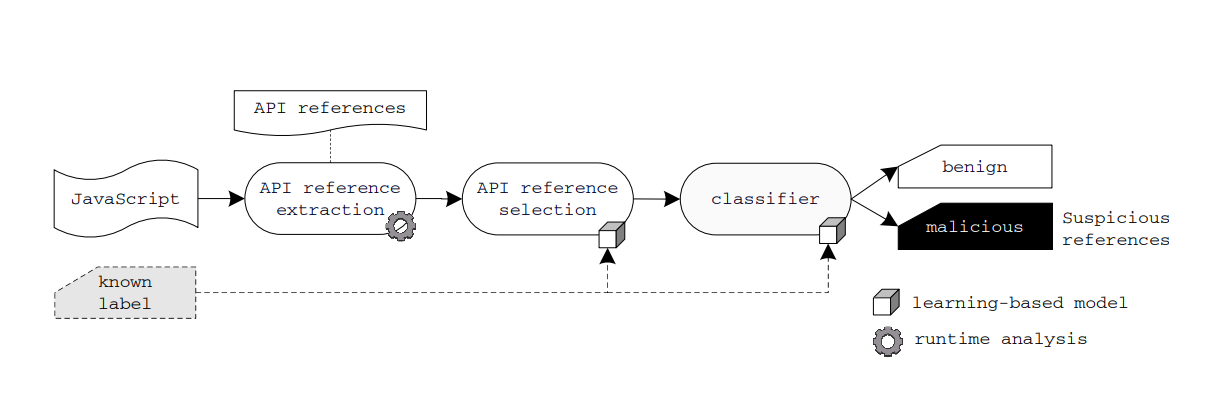
\includegraphics[width=\linewidth]{./images/luxOr.png}
	\caption{Mô hình kiến trúc của LuxOr \cite{luxor}}
	\label{fig:luxor}
\end{figure}

LuxOr sẽ thực hiện theo dõi tất cả các API javascript từ việc phân tích tĩnh và phân tích động. Sau đó, sẽ thông qua một quá trình lựa chọn API. Cuối cùng đưa ra một tập đặc trưng ứng với các API đã chọn để đưa vào quá trình phân loại. Hiện nay có các công cụ để trích xuất động API javascript như SpiderMokey hay Mozilla. Tuy nhiên những trình thông dịch như vậy nhận diện dựa trên tiêu chuẩn Js ECMA, không nhận diện được những API tương tác với trình đọc Acrobat Reader, ví dụ một số hàm như app.doc.syncAnnotScan(), app.plugIns.length, app.doc.getAnnots(). Do đó điểm nổi bật của LuxOr đã sử dụng công cụ PhoneyPdf được phát triển để giả lập và mô phỏng Adobe DOM, từ đó có thể thông dịch được các API Acrobat.

Kết quả thực nghiệm của LuxOr đã chứng minh rằng nó có hiệu quả trên rất nhiều các mẫu PDF chứa javascript, ngay cả với những CVE chứa những đoạn mã đã bị obfuscation. Có thể nói, công cụ này có thể được sử dụng phục vụ cho phát triển giai đoạn hai trong phương pháp phát hiện tài liệu PDF tôi đã đề xuất ở trên.

\end{document}

